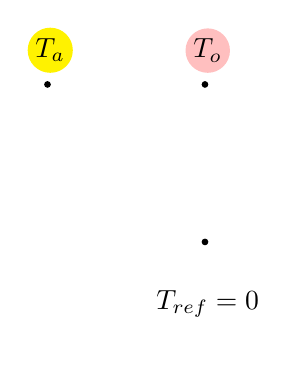
\begin{tikzpicture}
\draw (0,0) node[draw,fill,inner sep=0pt,outer sep=0pt,circle] (Ta) {$\rule{2pt}{0pt}$};
\draw (Ta.0) node[above=4pt,circle, inner sep=1pt,fill=yellow] {$T_{a}$};
\draw (2,0) node[draw,fill,inner sep=0pt,outer sep=0pt,circle] (To) {$\rule{2pt}{0pt}$};
\draw (To.0) node[above=4pt,circle, inner sep=1pt,fill=pink] {$T_{o}$};
%\draw (4,0) node[draw,fill,inner sep=0pt,outer sep=0pt,circle] (T1) {$\rule{2pt}{0pt}$};
%\draw (T1.0) node[above=4pt,circle, inner sep=1pt,fill=green] {$T_{1}$};
\draw (2,-2) node[draw,fill,inner sep=0pt,outer sep=0pt,circle] (Tref) {$\rule{2pt}{0pt}$};
\draw (Tref.0) node[below=2pt,circle,inner sep=1pt] {$T_{ref}=0$};

\end{tikzpicture}